\section{The Benchmarx Framework}
\label{sec:Benchmarx}

%\NOTE{\emph{Length:} 2 p., \emph{Responsible:} Thomas}
%
%\NOTE{Overview of the framework, provided components, approach to tool integration, synchronization dialogues, design and classification of test cases, execution of test cases.}
\subsection{Overview}

\begin{figure}[tb!]
	\centering
	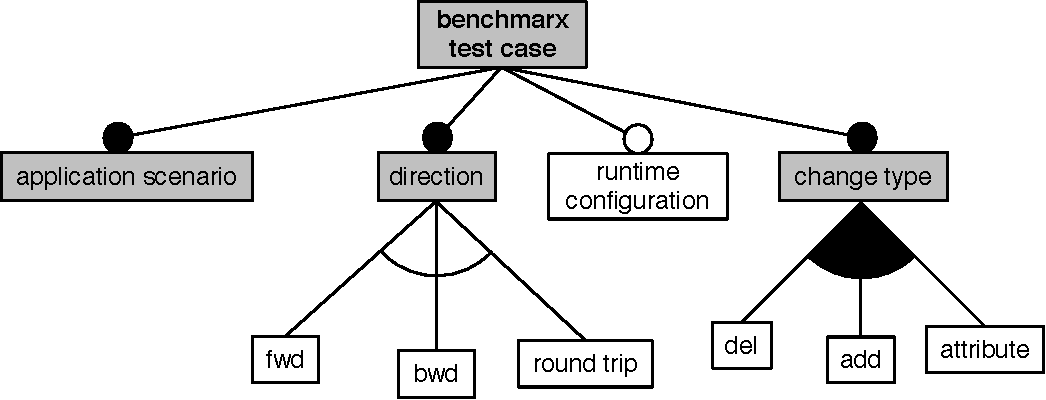
\includegraphics[width=\columnwidth]{diagrams/framework/feature-model-benchmarx-test-case}
	\caption{Variability of benchmarx test cases}
	\label{fig:featureModelBenchmarxTestCase}
\end{figure}

The Benchmarx framework is a component-based framework allowing for a comparison of arbitrary BX tools. The major challenge in benchmarking bx tools is that different tools may use different input data. Addressing this challenge requires a unifying design space, in which different tool architectures can be placed and respectively classified. 

The framework is based on Eclipse EMF technology, but it is also open to bx tools operating on plain Java Objects and even non-JVM based tools. JUnit test cases are used to setup and execute the benchmarx tests. Assertions ensure the respective pre- and postconditions and the expected transformation results. In order to compare the expected and the actual resulting target models of each transformation run, a string representation of the respective models is used. In that way, non-EMF and even non-JVM-based tools may be used and no restrictions on the input data of the tools considered are imposed. 

\subsection{Design of the Test Cases}

As an extension of the feature model for bx tool architectures, Figure \ref{fig:featureModelBenchmarxTestCase} depicts a feature model for benchmarx test cases. Every benchmarx test case must state the required bx tool architecture (c.f. Fig. \ref{fig:featureModelBxTools}), its direction to be \textbf{fwd} (forward), \textbf{bwd} (backward) or \textbf{round trip}, and the combination of different change types applied in the test. The set of possible change types can be extended in the future to accommodate more expressive frameworks. 

The test cases provided for the Families to Persons case are separated into two different categories: (1) batch test cases and (2) incremental ones. Each category comprises test cases for each transformation direction. Please note that in the following the term \emph{forward} is used for transformations from the Families model to the Persons model. Accordingly, a \emph{backward} transformation describes a transformation from the Persons model to the Families model.

While the batch test cases are used to check if a given source model is transformed into a target model correctly, updates of the corresponding source models are taken into account by the incremental ones. In particular, renaming, deleting and moving persons and family members respectively, are addressed in these test cases. In order to keep the number of test cases manageable, only the batch category contains separate test cases for each combination of configuration parameters. In the incremental category, the parameters are changed dynamically during test case execution.

Benchmarx is designed as a generic framework for benchmarking BX tools, and -- as stated above -- not all of the tools provide access to internal data structures like correspondence models or output deltas of a synchronization run, the JUnit test cases are designed as \emph{synchronisation dialogues}. They always start from the same agreed upon consistent state, from which a sequence of deltas are propagated. Only the resulting output models are to be directly asserted by comparing them with expected versions. 

A benchmarx test case is depicted schematically to the left of Figure \ref{fig:benchmarxTestCase}, with a concrete test case for our example to the right, following the proposed structure and representing an instantiation with JavaDoc, Java, and JUnit.

\begin{figure}[tb!]
	\centering
	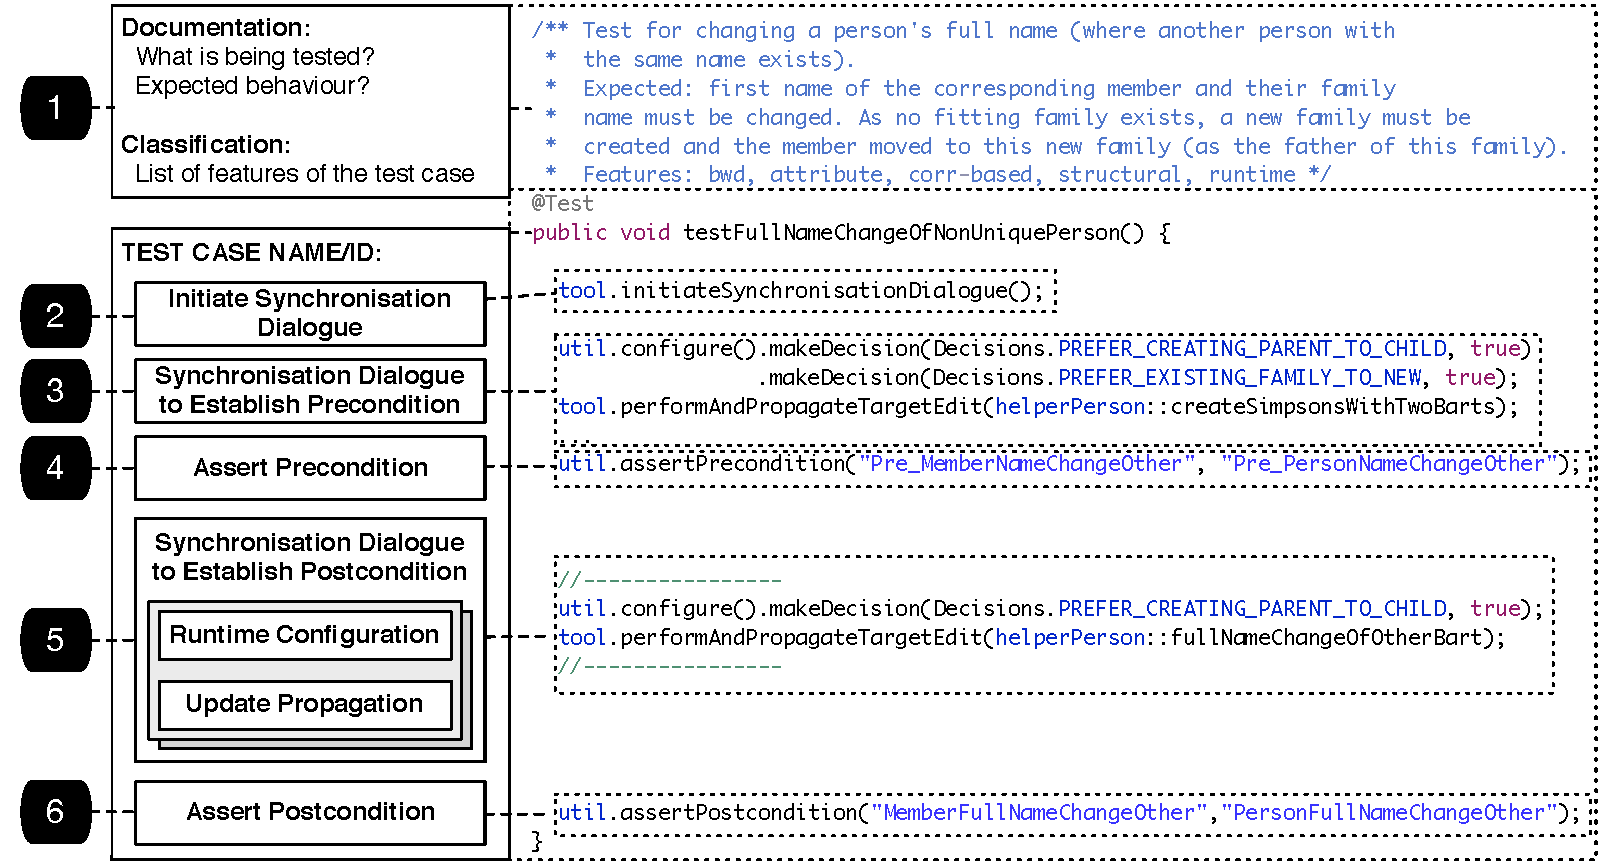
\includegraphics[width=\columnwidth]{diagrams/testCase}
	\caption{A benchmarx test case as a synchronisation dialogue}
	\label{fig:benchmarxTestCase}
\end{figure}

Each test case contains a documentation (cf. Label 1 in Figure \ref{fig:benchmarxTestCase}) stating (i) what is being tested, (ii) the expected behaviour, and (iii) a list of the concrete features of the test case taken from Figure \ref{fig:featureModelBenchmarxTestCase} to clarify at a glance if a given bx tool can pass the test or not. 

The test case itself starts with an initialisation command invoked on the bx tool which is being tested (Label 2), where the agreed upon starting state is established (e.g., for the Families to Persons benchmarx this comprises a single empty family register and a corresponding single empty person register), and all neccessary internal (auxiliary) data structures are created.

Part three (Label 3) of a test case consists of a series of propagation steps, used to establish the precondition of the test. Although this creates a dependency to other tests (asserting exactly this precondition), the handling of the required correspondence model is simplified, as the bx tool can build up the neccessary internal state that must go along with the precondition. I.e. the old consistent correspondence model is ``passed'' implicitly to the bx tool via a series of preparatory propagation steps. The precondition is finally asserted (Label 4), representing a well-defined starting point. If the test requires a runtime update policy, this is configured just before propagating the actual input delta (Label 5). The last part of a test case (Label 6) is an assertion of the postcondition, checking if the final source and target models are as expected. 

In the concrete test case shown in Figure \ref{fig:benchmarxTestCase}, a number of persons are created in the person register and then propagated backward to establish a consistent family register that is asserted as a precondition. As part of the actual test, a person named \texttt{Simpson, Bart} is now renamed in the person register; this change is now propagated backward with the update policy to prefer creating parents (if possible) to creating children. Please note that in this test scenario multiple persons with the name \emph{Bart Simpson} are used. As a consequence, the respective correspondences between those persons and their counterparts in the family model need to be managed.

\subsection{Implementation in a Tool}

In order to use a specific bx tool with the benchmarx framework, the interface \code{BXTool} needs to be implemented. Please note, although the Benchmarx Framework itself is written in Java, it is possible to also use it with non-JVM based BX tools (c.f, our reference implementation for the tool BiGUL). Figure \ref{fig:refImplementation} gives an overview and explanation of the methods to be implemented. Reference implementations for \emph{eMoflon} \cite{}, \emph{BiGUL} \cite{}, \emph{medini QVT}\footnote{http://projects.ikv.de/qvt} and \emph{BXtend} \cite{MODELSWARD2018-Buchmann} may be found in the benchmarx Github repository. Please note that for EMF-based tools, an abstract class \code{BXToolForEMF} already exists where tool integrators may subclass from. This class already contains implementations for both \code{assert} methods. As explained in the previous subsection, the method \code{initiateSynchronisationDialogue} is invoked on each test case run and is used to establish the agreed upon common starting state consisting of a single empty family register and its corresponding single and empty persons register plus all neccessary and tool-specific internal data structures. The methods \code{performAndPropagateTargetEdit} and \code{performAnd-\\} \code{PropagateSourceEdit} are called from the test cases when corresponding edit deltas should be performed and propagated on the corresponding models. In contrast, the methods \code{performIdleTargetEdit} and \code{per\-formIdleSourceEdit} are used to modify source and target models, respectively, without propagating the change. These methods should be used whenever a change in the respective models does not affect the opposite model, e.g. when the birthday date of a person is changed, or the role of a family member within its containing family.

Please note, that we use parameterized test cases, where the \code{BXTool}s are the parameters. In order to run the test cases for a single tool, the respective test runner has to be instantiated in the corresponding collection the class \code{FamiliesToPersonsTestCase}. 

\begin{figure}[tb!]
	\centering
	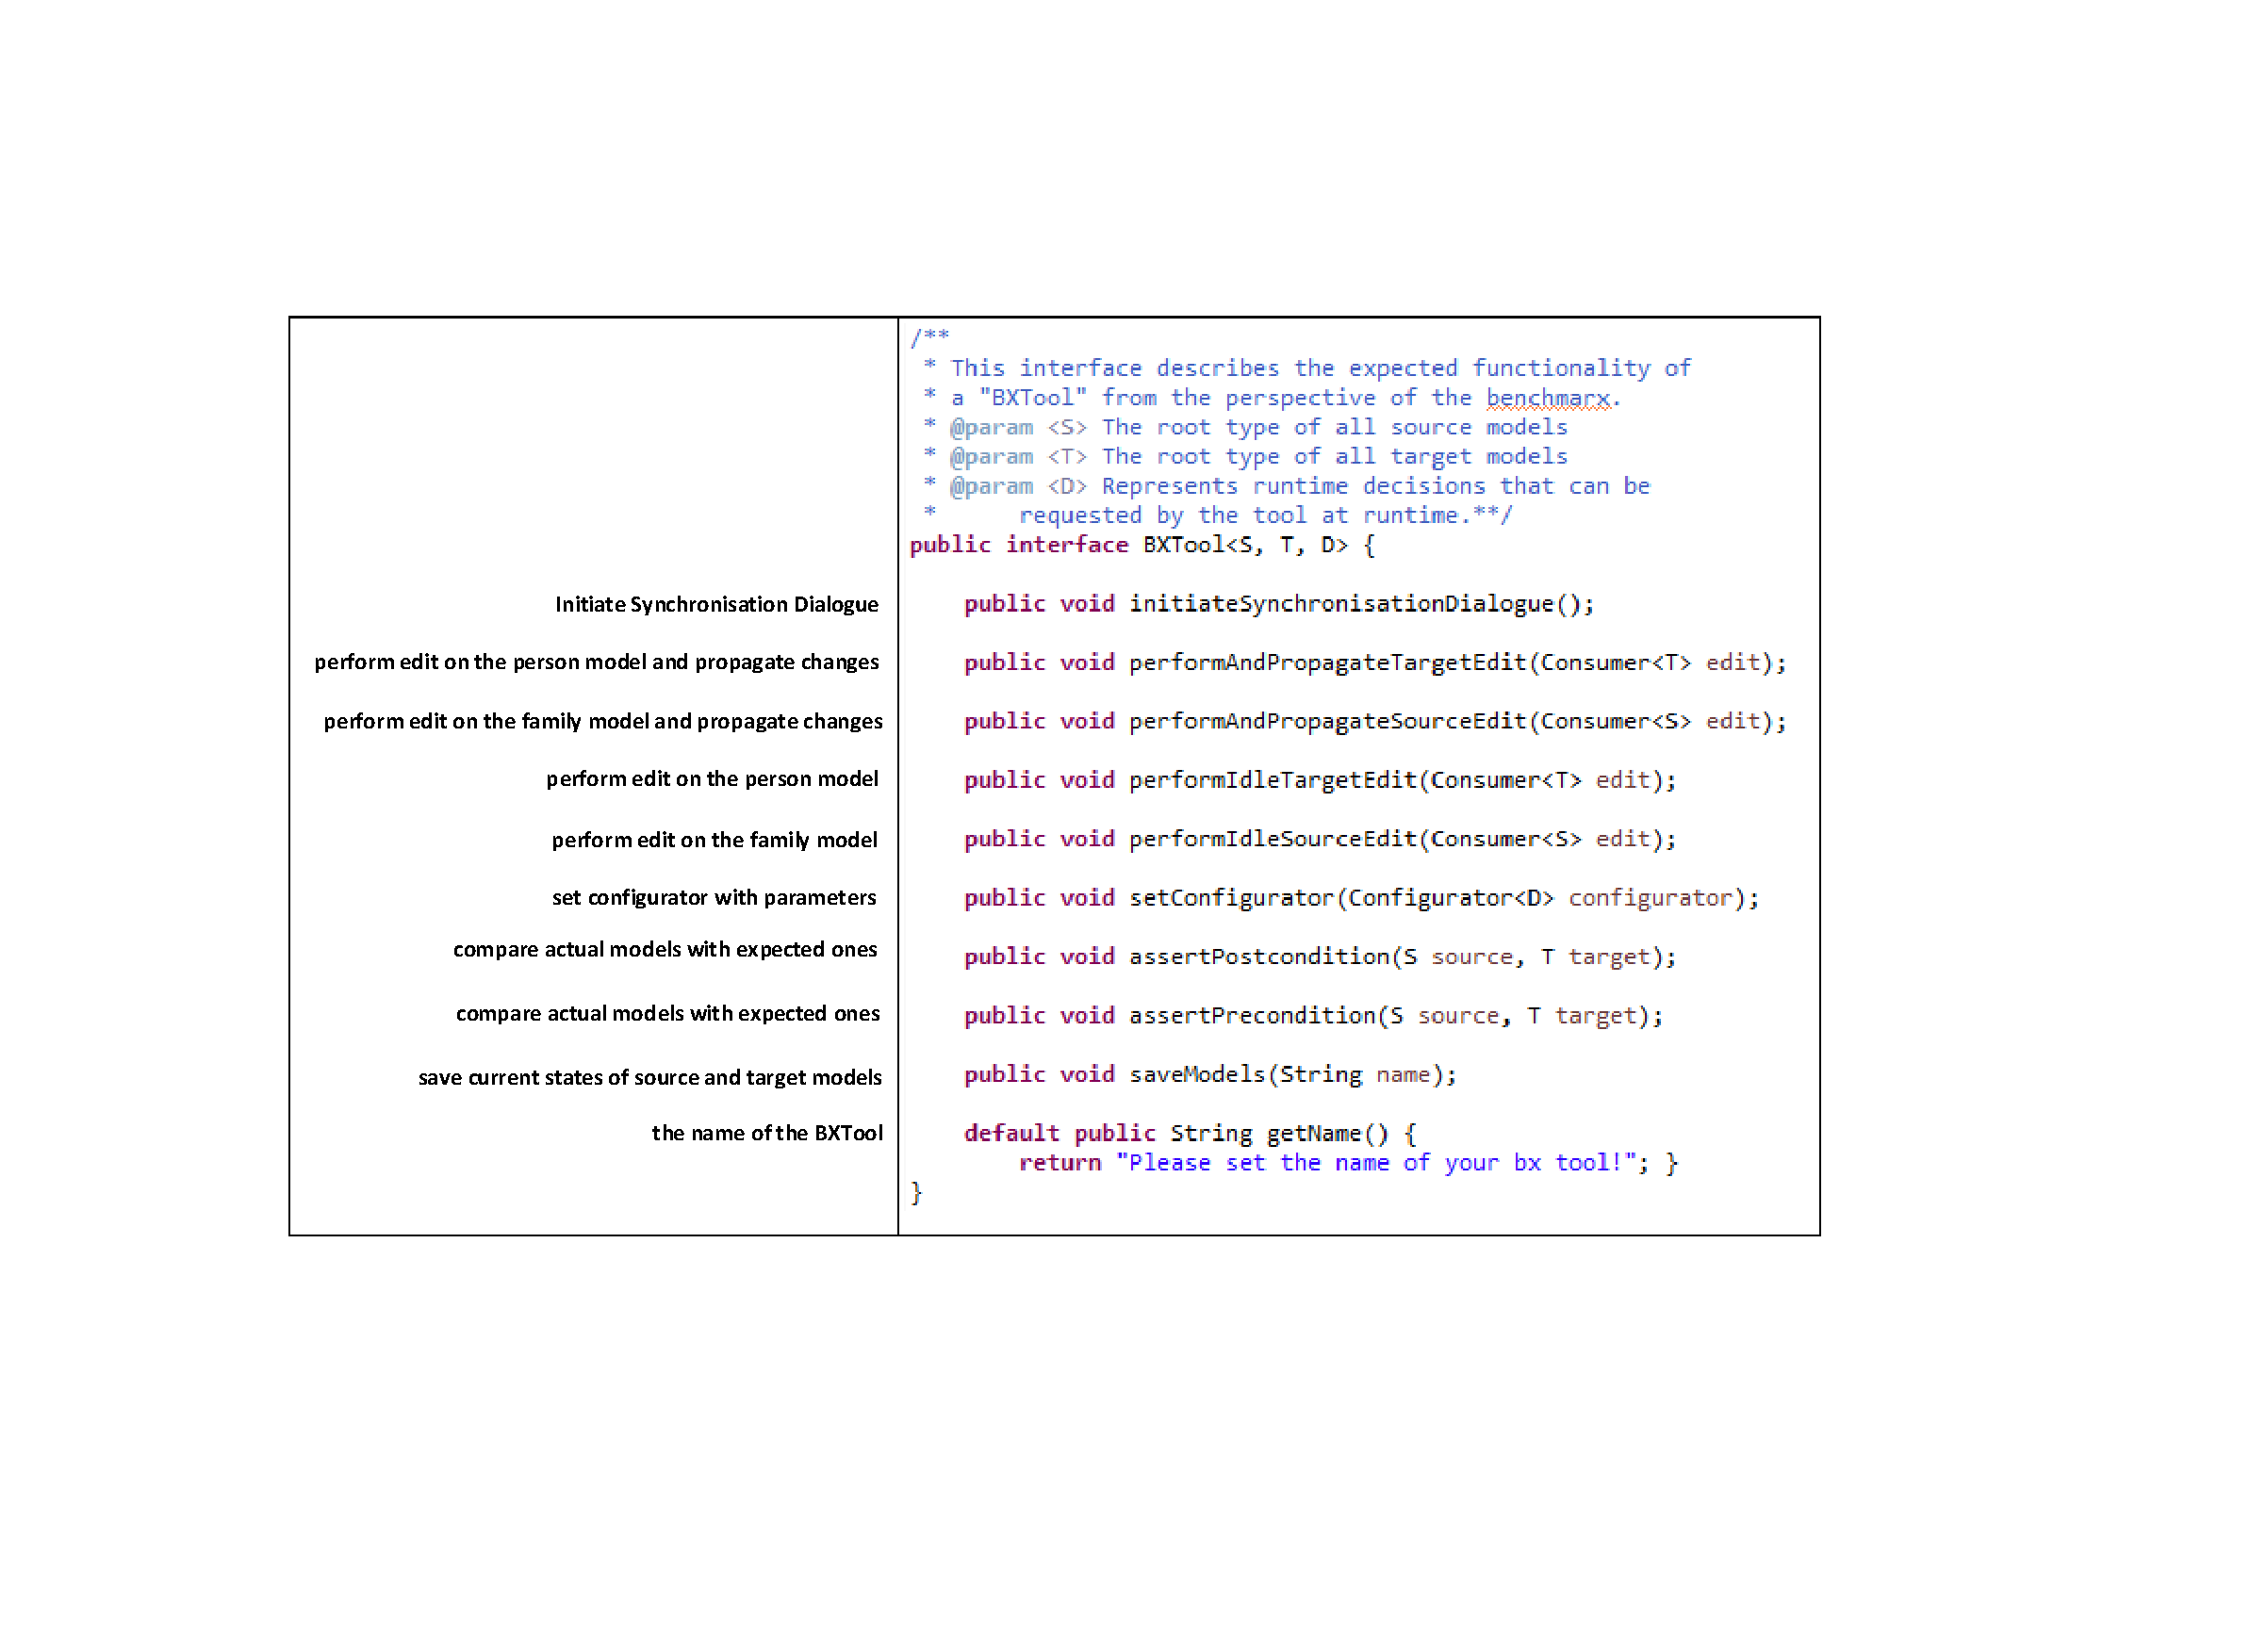
\includegraphics[width=\columnwidth]{diagrams/BXTool}
	\caption{The BXTool interface.}
	\label{fig:refImplementation}
\end{figure}



